%=================AVANCES Y PRUEBAS=================
% SENSORES DE PULSO

\section{Módulo Autenticación}
Para que el usuario pueda acceder a la funcionalidad de la app, es necesario que siga uno de los flujos establecidos, los cuales se describen a continuación.\\


\subsection{Login}

La figura \ref{fig:SecuenciaLogin} se muestra el diagrama de secuencia correspondiente al login del usuario, mismo que contiene los métodos implementados en la clase JAVA, API e IU.

\begin{figure}[htbp!]
	\centering
	\fbox{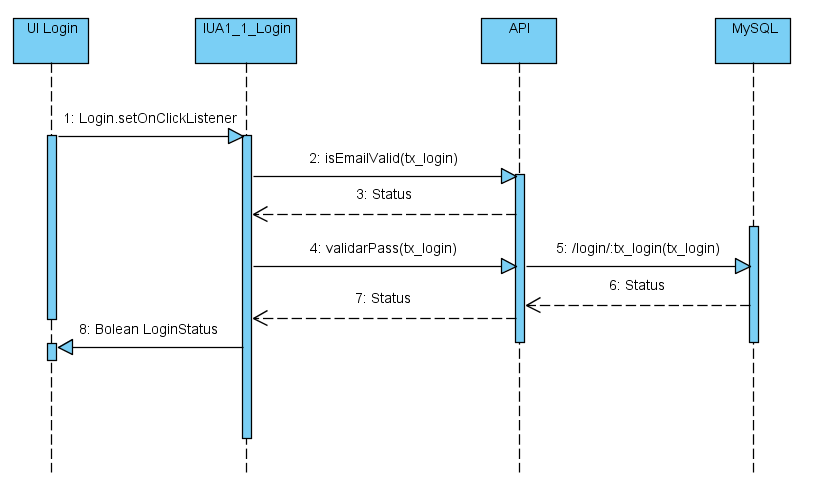
\includegraphics[width=0.9\textwidth]{AvancesPruebas/imagenes/SecuenciaLogin}}
	\caption{Diagrama secuencia Login}
	\label{fig:SecuenciaLogin}
\end{figure}
\begin{itemize}
	\item \textbf{Login.setOnClickListener:} Es la acción que dispara el usuario, no recibe datos como parámetros, es el disparador.
	\item \textbf{isEmailValid(tx login):} Valida que el correo electrónico sea válido, se realiza la validación con base en una expresión regular.
	\item \textbf{validarPass(tx login):} Dispara una petición al API, enviando como parámetro el correo del usuario, esto para obtener el password correspondiente al correo electrónico.
	\item \textbf{/login/:tx login:} Es la ruta para la obtención del password correspondiente al correo electrónico.
\end{itemize}

\subsection{Recuperar Contraseña}

La figura \ref{fig:SecuenciaRecupera} se muestra el diagrama de secuencia correspondiente a la recuperación de cuenta del usuario, mismo que contiene los métodos implementados en la clase JAVA, API e IU.

\begin{figure}[htbp!]
	\centering
	\fbox{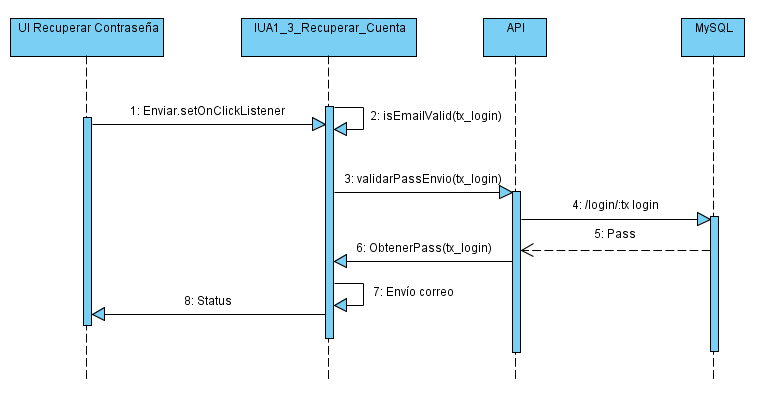
\includegraphics[width=0.9\textwidth]{AvancesPruebas/imagenes/SecuenciaRecupera}}
	\caption{Diagrama secuencia Recuperar Contraseña}
	\label{fig:SecuenciaRecupera}
\end{figure}

\begin{itemize}
	\item \textbf{Enviar.setOnClickListener:} Es la acción que dispara el usuario, no recibe datos como parámetros, es el disparador.
	\item \textbf{isEmailValid(tx login):}  Valida que el correo electrónico sea válido, se realiza la validación con base en una expresión regular.
	\item \textbf{validarPassEnvio(tx login):} Envía al API la solicitud para consulta de correo para saber si existe, manda como parámetro el correo electrónico ingresado por el usuario.
	\item \textbf{ObtenerPass(tx login):} Obtiene el password del correo electrónico que se manda como parámetro.
	\item \textbf{/login/:tx login:} Es la ruta para la obtención del password correspondiente al correo electrónico. 
\end{itemize}



\subsection{Registro de Cuenta}
La figura \ref{fig:SecuenciaCuenta} se muestra el diagrama de secuencia correspondiente al registro de cuenta del usuario, mismo que contiene los métodos implementados en la clase JAVA, API e IU.
\begin{figure}[htbp!]
	\centering
	\fbox{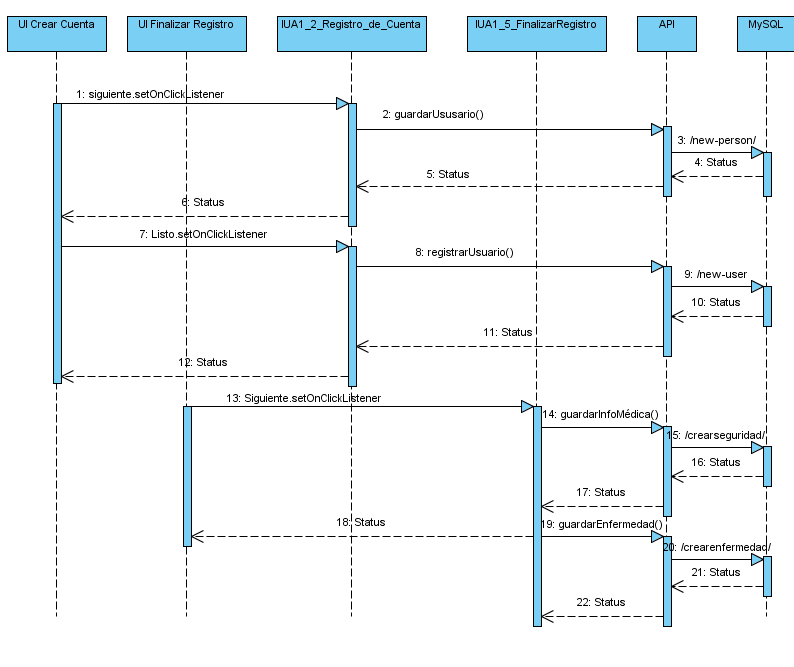
\includegraphics[width=0.9\textwidth]{AvancesPruebas/imagenes/SecuenciaCuenta}}
	\caption{Diagrama secuencia Crear Cuenta}
	\label{fig:SecuenciaCuenta}
\end{figure}

\begin{itemize}
	\item \textbf{siguiente.setOnClickListener:} Es la acción que dispara el usuario, no recibe datos como parámetros, es el disparador.
	\item \textbf{guardarUsusario():} Este método realiza las validaciones correspondientes a las RN para poder guardar una persona.
	\item \textbf{/new-person/:} Es la ruta para el registro de una nueva persona en la base de datos.
	\item \textbf{Listo.setOnClickListener:}  Es la acción que dispara el usuario, no recibe datos como parámetros, es el disparador.
	\item \textbf{registrarUsuario():} Este método realiza las validaciones correspondientes a las RN para poder guardar un usuario.
	\item \textbf{/new-user:} Es la ruta para el registro de una nueva cuenta en la base de datos
	\item \textbf{Siguiente.setOnClickListener:} Es la acción que dispara el usuario, no recibe datos como parámetros, es el disparador.
	\item \textbf{guardarInfoMédica():} Este método realiza las validaciones correspondientes a las RN para poder guardar la información médica de la persona.
	\item \textbf{/crearseguridad/:} Esta ruta permite registrar la información médica del usuario.
	\item \textbf{guardarEnfermedad():} Este método realiza las validaciones correspondientes a las RN para poder guardar la información de enfermedad de la persona.
	\item \textbf{/crearenfermedad/:} Esta ruta permite registrar la información de enfermedad del usuario.
\end{itemize}


